\documentclass[12pt,a4paper]{report}
\usepackage[T1]{fontenc}
\usepackage[utf8]{inputenc}
\usepackage[romanian]{babel}
\usepackage{times}
\usepackage{graphicx}
\usepackage{enumitem}
\usepackage{fancyhdr}
\usepackage{geometry}
\usepackage{float}

\geometry{
	a4paper,
	total={165mm,245mm},
	left=22mm,
	top=25mm,
}

\newcommand{\uline}[1]{\rule[0pt]{#1}{0.4pt}}

\pagestyle{fancy}
\setlength{\voffset}{-24pt}
\setlength\headheight{54.0pt}
\renewcommand{\headrulewidth}{0pt}
\chead{%
	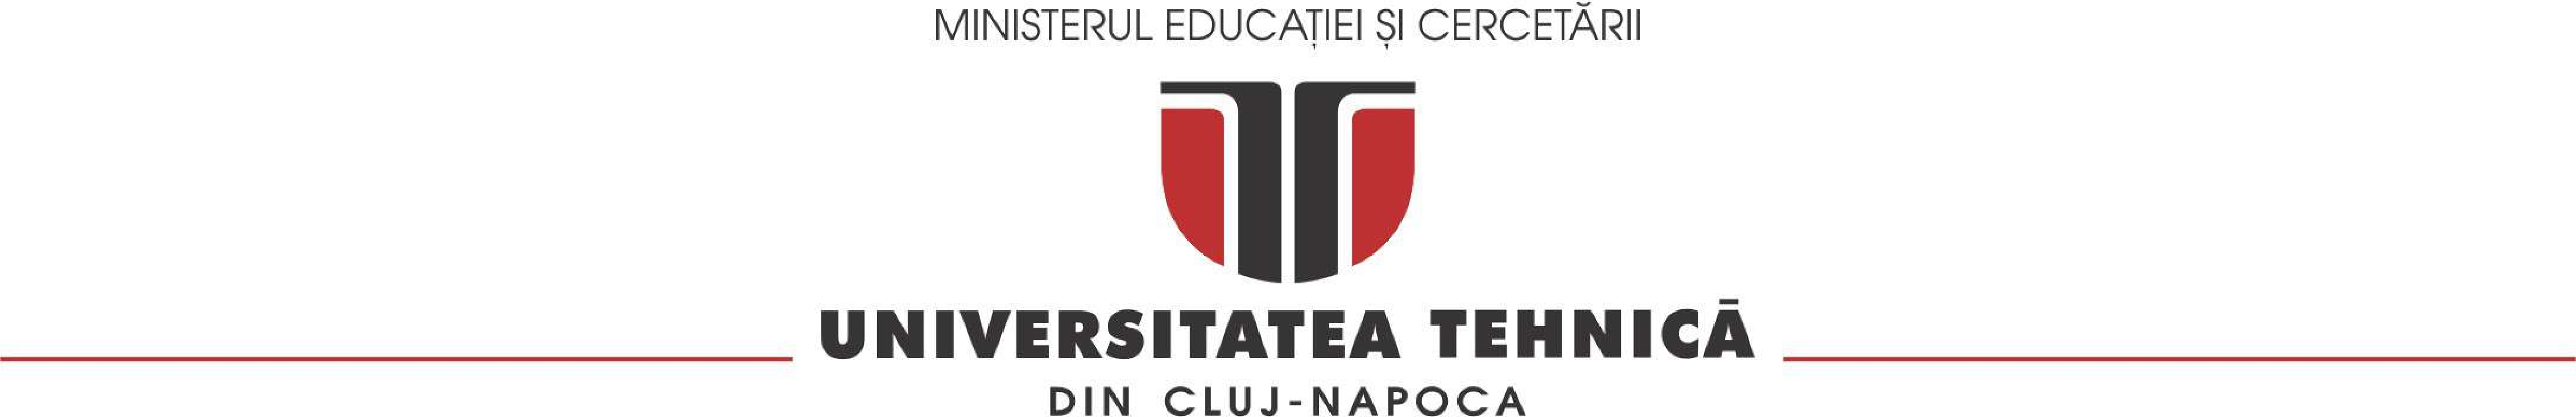
\includegraphics[width=\textwidth]{figs/AntetUTCNRom.pdf}
}
\cfoot{}
\lfoot{}
\rfoot{}

\setlength{\parindent}{1.2em}

\newcommand{\figcap}[1]{\\[2pt]{\footnotesize\itshape #1}}

\begin{document}

\begin{center}
	{\sffamily\bfseries\small FACULTATEA DE AUTOMATICĂ ȘI CALCULATOARE\\
	DEPARTAMENTUL CALCULATOARE}

	\vspace{0.3cm}

	SINTEZA\\
	proiectului de diplomă cu titlul:

	\vspace{0.3cm}

	{\large\scshape Sistem de Control FPGA pentru Mână Robotică cu Filtrare Kalman}
\end{center}

\vspace{0.4cm}

\noindent
\begin{tabular}{@{}p{3cm}l@{}}
	Autor: & {\bf Radu-Rareș CIOBANU}\\
	Coordonator: & {\bf Prof. dr. ing. Radu Gabriel DĂNESCU}\\
\end{tabular}

\vspace{0.5cm}

\begin{enumerate}[leftmargin=1.3cm]

\item \textbf{Cerințele temei:}

Cerința principală a temei a constat în proiectarea și implementarea părții de control,
pe o placă FPGA, a unui sistem capabil să acționeze în timp real o mână robotică cu opt
servomotoare, astfel încât aceasta să reproducă mișcările mâinii umane.

Din punct de vedere funcțional, sistemul trebuie să primească unghiurile articulațiilor
prin interfața serială UART, să filtreze zgomotul acestor comenzi, să genereze cele opt
semnale de comandă de tip PWM și să citească poziția reală a servomotoarelor printr-un
convertor analog-digital. Pe lângă aceste funcții, sistemul trebuie să funcționeze fără
întreruperi în timp real pe un circuit de 100~MHz, să păstreze partea logică izolată
galvanic de zgomotul electric al servomotoarelor și să realizeze toate calculele în
aritmetică cu virgulă fixă, întrucât circuitul nu dispune de o unitate în virgulă mobilă.

\item \textbf{Soluții alese:}

Sistemul propus funcționează ca o buclă închisă de control, având rolul de a prelua
comenzile din mediul digital, de a le netezi și de a le transmite către servomotoare,
citind totodată poziția reală a acestora. Din punct de vedere arhitectural, partea
digitală este structurată în module logice interconectate, descrise în VHDL, pentru
recepția și validarea cadrelor UART, sincronizarea printr-un modul de tip mailbox, filtrarea
Kalman, generarea PWM și bucla de achiziție prin convertorul analog-digital. Această
organizare este reprezentată în Figura~2.1.

\begin{figure}[H]
	\centering
	
\includegraphics[width=0.88\textwidth]{figs/bw/arhitectura_module.png}
	\figcap{Figura 2.1 --- Arhitectura modulelor VHDL implementate pe placa Basys3.}
\end{figure}

Nucleul soluției îl reprezintă un filtru Kalman cu două stări, poziție și viteză,
realizat integral în aritmetică cu virgulă fixă Q16.16 și capabil să prelucreze toate
cele opt canale într-un singur ciclu de control. Împărțirea necesară pasului de corecție
este realizată pe mai multe cicluri de ceas, printr-un modul dedicat de tip restoring
divider, pentru a respecta constrângerile temporale. Comanda rezultată din filtrare este
transformată apoi în semnale PWM cu lățime între 0,544~ms și 2,4~ms, corespunzătoare
cursei complete a servomotoarelor. Pe latura fizică, izolarea galvanică este asigurată de două izolatoare
ADuM1400 pe calea de comandă și de izolatorul SPI MAX14850 pe calea de măsurare.
Convertorul analog-digital AD7124-8, pe 24 de biți, citește poziția servomotoarelor prin
divizoare rezistive, iar alimentarea de precizie este furnizată de modulul DC2468A
împreună cu regulatorul liniar ADP165. Ansamblul conexiunilor este prezentat în
Figura~2.2.

\begin{figure}[H]
	\centering
	\includegraphics[width=0.78\textwidth]{figs/bw/schema_conexiuni.pdf}
	\figcap{Figura 2.2 --- Schema conexiunilor dintre placă, izolatoare, convertor și servomotoare.}
\end{figure}

\item \textbf{Rezultate obținute:}

Rezultatul principal al proiectului constă în realizarea cu succes a părții de control pe
placa FPGA, împreună cu integrarea acesteia în ansamblul mecanic al mâinii robotice.
Partea digitală funcționează corect și stabil, respectând toate constrângerile temporale,
iar mâna reproduce mișcările comandate și reușește să prindă și să susțină obiecte reale.
Bucla de feedback citește corect toate cele opt canale ale convertorului analog-digital,
iar integrarea părții mecanice cu cea digitală a funcționat de la prima încercare, ceea ce
validează abordarea de testare pe niveluri. Ansamblul fizic realizat, împreună cu montajul
de comandă, este prezentat în Figura~3.1.

\begin{figure}[H]
	\centering
	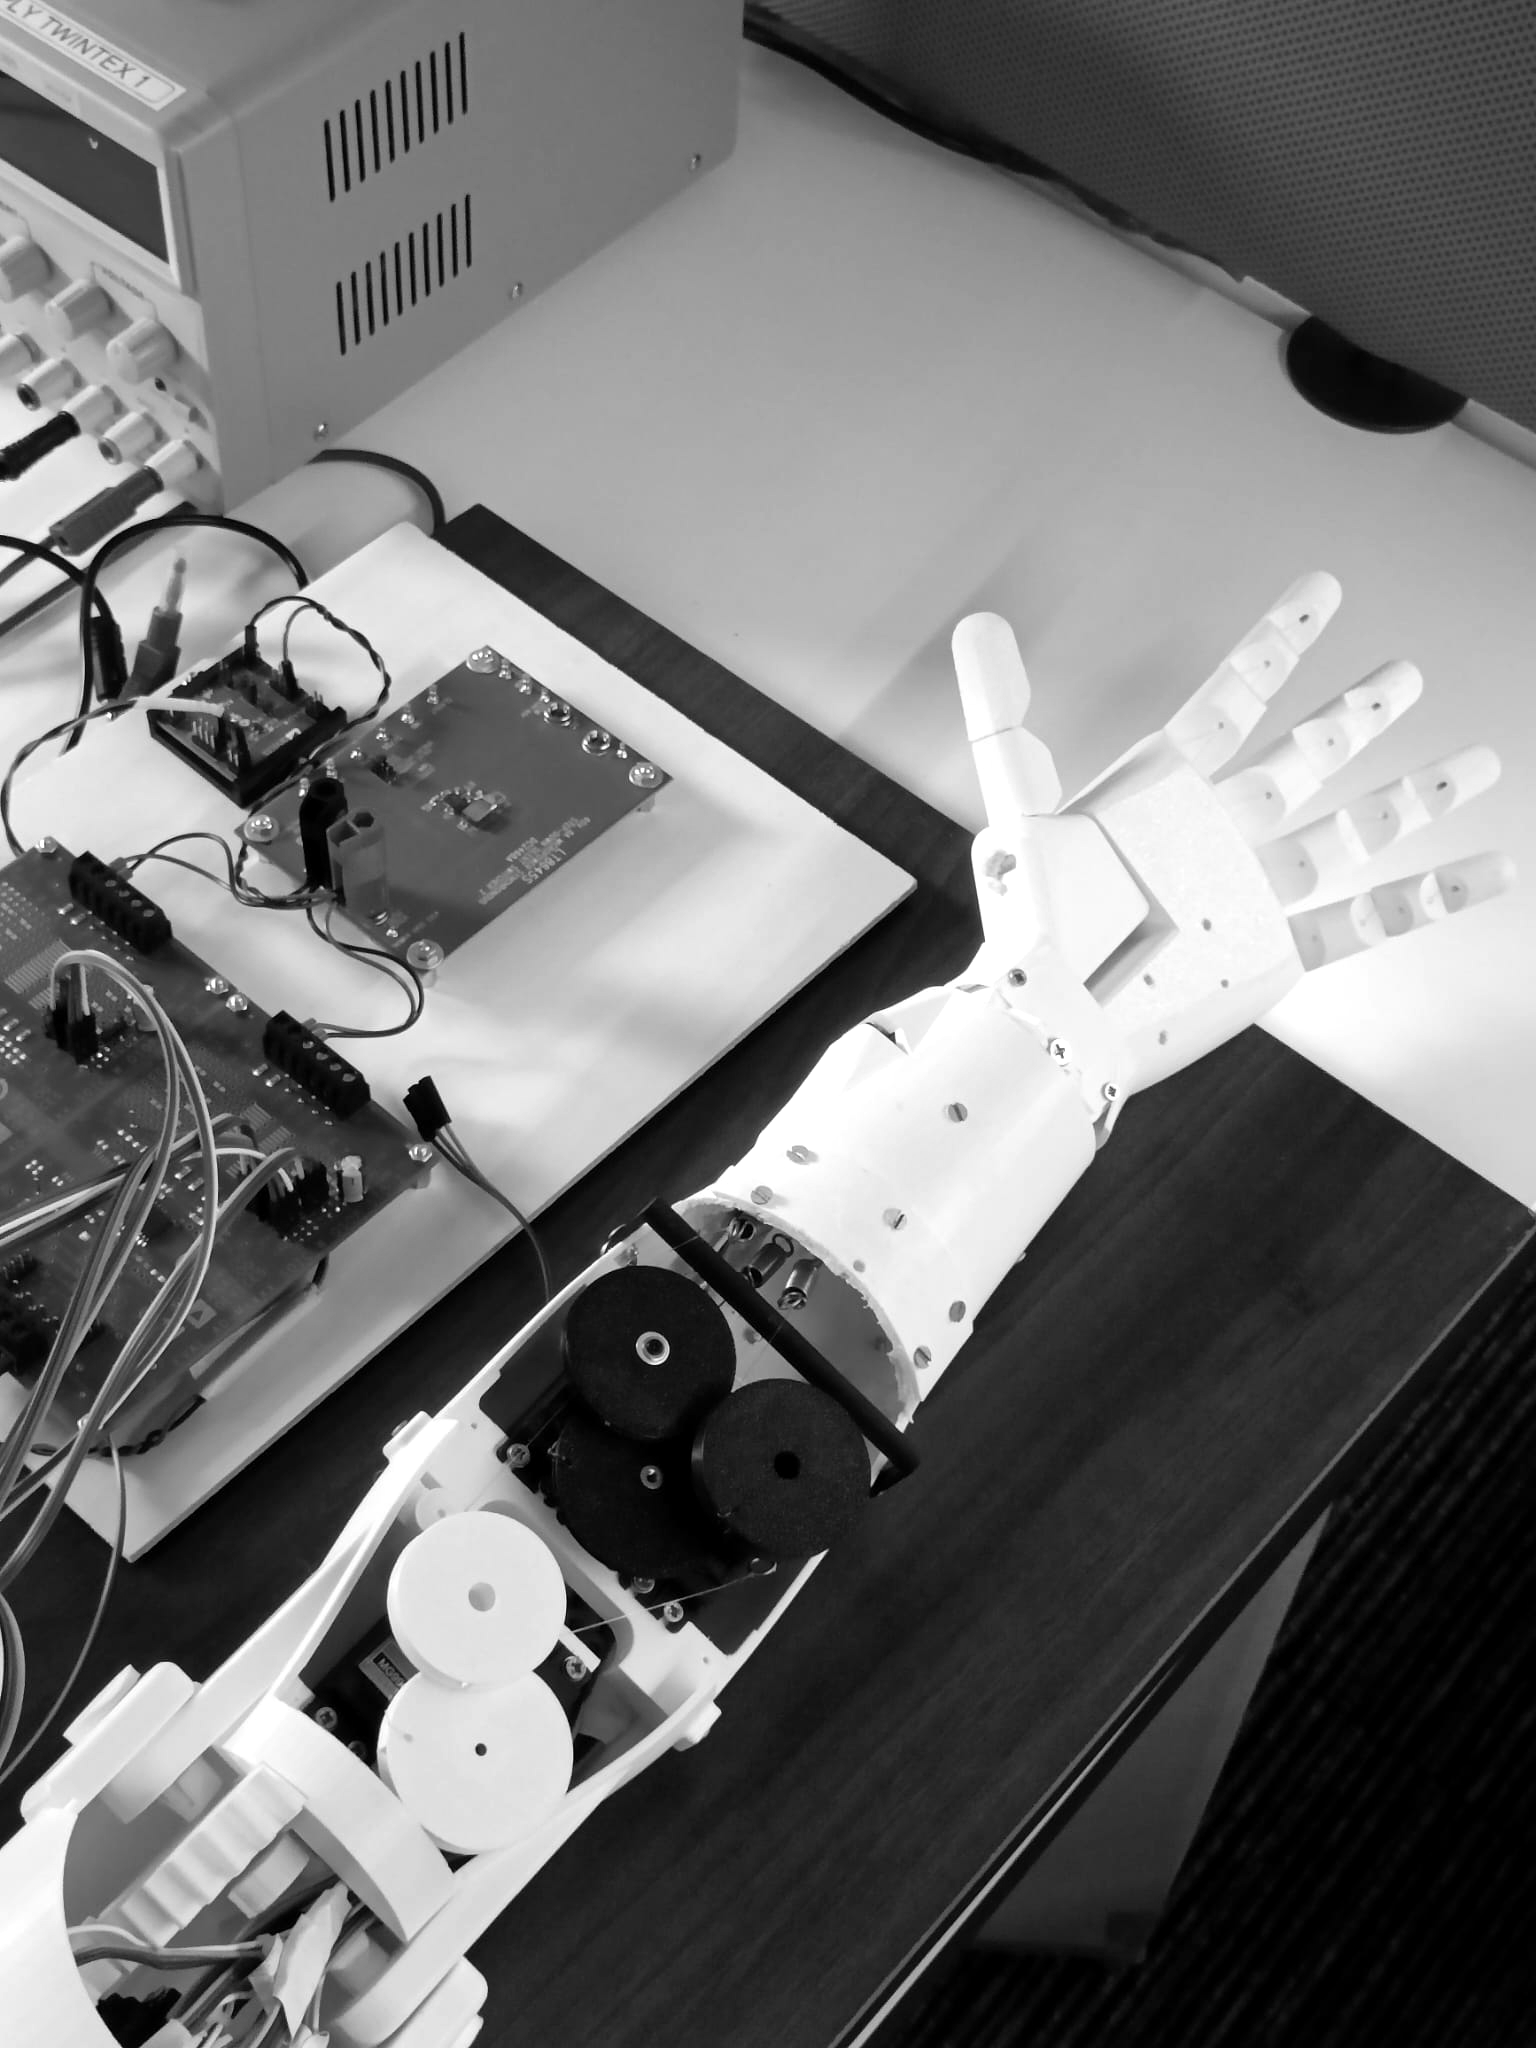
\includegraphics[height=6.5cm]{figs/bw/brat_real.png}
	\figcap{Figura 3.1 --- Mâna robotică realizată, împreună cu placa FPGA și montajul de alimentare.}
\end{figure}

\item \textbf{Testări și verificări:}

Evaluarea a urmat o abordare pe niveluri, în care fiecare modul a fost verificat separat
înainte de integrare, pornind de la generatoarele PWM și filtrul Kalman și continuând cu
lanțul complet de comandă și feedback. Respectarea constrângerilor temporale la 100~MHz a
fost confirmată prin raportul de analiză temporală din mediul Xilinx Vivado. Comunicația
SPI cu convertorul a fost verificată cu ajutorul unui osciloscop, care a permis
observarea directă a semnalelor de pe magistrală și confirmarea citirii corecte a
registrului de identificare și a celor opt canale de conversie.

\item \textbf{Contribuții personale:}

Contribuția centrală a acestei lucrări o reprezintă implementarea părții de control pe
placa FPGA. Din punct de vedere algoritmic, a fost proiectat și implementat un filtru
Kalman cu două stări în aritmetică cu virgulă fixă Q16.16, adaptat unei platforme fără
unitate în virgulă mobilă. Închiderea temporală a circuitului a impus descompunerea
operațiilor complexe, realizarea împărțirii pe mai multe cicluri de ceas și distribuirea
stării filtrului în memorii separate.

Pe latura de comunicație, a fost dezvoltat un lanț complet de prelucrare, de la recepția
și validarea cadrelor prin UART, cu sumă de control, până la mecanismul de sincronizare
de tip mailbox și generarea celor opt semnale PWM. Bucla de feedback prin SPI a
necesitat proiectarea unui controler dedicat pentru convertorul AD7124-8, respectând
protocolul acestuia și modul de operare peste bariera de izolare.

Dincolo de partea digitală, o contribuție importantă o constituie realizarea fizică a
mâinii, gândită ca un ansamblu care îmbină mai multe soluții existente cu piese proiectate
și modelate special pentru acest proiect. La aceasta se adaugă integrarea componentelor
Analog Devices, folosite pentru izolarea galvanică, achiziția de precizie și alimentarea
stabilă a întregului sistem.

\item \textbf{Surse de documentare:}

\begin{itemize}[leftmargin=1.2em,itemsep=1pt,topsep=2pt]
	\item \textbf{R. E. Kalman}. \textit{A New Approach to Linear Filtering and Prediction
	Problems}. Sursa fundamentală pentru modelul teoretic al filtrului implementat.
	\item \textbf{Analog Devices}. \textit{AD7124-8, MAX14850, ADuM1400, ADP165 Datasheets}.
	Documentația tehnică a componentelor folosite pentru achiziție, izolare și alimentare.
	\item \textbf{Google}. \textit{MediaPipe Hands}. Resursă pentru urmărirea mâinii prin
	viziune, sursa unghiurilor transmise plăcii.
	\item \textbf{Digilent}. \textit{Basys3 Reference Manual}. Referința pentru placa FPGA și
	maparea pinilor.
	\item \textbf{Proiecte open-source} (InMoov și alte modele de mâini robotice). Surse de
	inspirație pentru ansamblul mecanic și sistemul de acționare prin tendoane.
\end{itemize}

\end{enumerate}

\vspace{0.1cm}

\noindent
\begin{tabular}{@{}p{7.5cm}@{}r@{~}l@{}}
	Data: 10.07.2026 & Autor & \rlap{\makebox[5cm][c]{\raisebox{0.02cm}{
\includegraphics[width=1.1cm]{figs/semnatura_trim.png}}}}\uline{5cm}\\[0.4cm]
	& Coordonator & \uline{5cm}\\
\end{tabular}

\end{document}
